\documentclass[a4paper,review,12pt]{elsarticle}

\usepackage[utf8]{inputenc}
\usepackage[T5]{fontenc}
\usepackage{amsmath}
\usepackage{amssymb}
\usepackage{booktabs}
\usepackage{tabularx}
\usepackage{array}
\usepackage{graphicx}
\usepackage{xcolor}
\usepackage{float}
\usepackage{microtype}
\usepackage{xurl}
\usepackage[hidelinks]{hyperref}

\definecolor{paceblue}{HTML}{0072B2}
\definecolor{pacesky}{HTML}{56B4E9}
\definecolor{pacegreen}{HTML}{009E73}
\definecolor{paceorange}{HTML}{E69F00}
\definecolor{pacevermillion}{HTML}{D55E00}
\definecolor{pacepurple}{HTML}{CC79A7}

\journal{Image and Vision Computing}

\newcommand{\method}{PACE-Seg}
\newcommand{\miou}{mIoU}
\newcommand{\etal}{et al.}
\setlength{\emergencystretch}{2em}

\begin{document}

\begin{frontmatter}

\title{PACE-Seg: Hardware-Cost-Conditioned Elastic Semantic Segmentation with Calibrated Risk Routing for Edge Accelerators}

\author{D\~{u}ng Nguy\~{\^{e}}n}

\begin{abstract}
Edge semantic segmentation faces two coupled uncertainties: visual difficulty changes under adverse conditions, and model cost changes across accelerator architectures. We present \method, a compiler-safe elastic model with four statically deployable capacities and a runtime policy that combines measured route latency with candidate-specific error estimates from one low-cost entropy probe. Experiments use Cityscapes, four ACDC conditions, and four edge devices. The capacities span $110.2\times$ in FLOPs but only $10.3$--$19.5\times$ in measured candidate latency, so a proportional FLOPs proxy fails to reproduce measured budget choices. The largest elastic capacity remains within 1.1 \miou{} points of a similarly sized independently trained Fast-SCNN on every evaluated split. In deployment-matched held-out replay with complete warm-route costs on TensorRT/CUDA and Hailo-8, the budget-constrained policy outperforms or matches rank escalation in 70 of 74 fair operating cells, with a macro gain of 0.0284 \miou{}; it produces no budget-violating cell, compared with 46 of 120 for rank escalation. Pooled calibration gives a similar result, indicating that the gain does not require condition-specific calibrator selection. These cells are correlated evaluations, and the two backends share segmentation predictions. A secondary fake-quant study keeps worst-condition degradation within 1.5 \miou{} points for every tested run and elasticity level but does not establish compiled INT8 accuracy.
\end{abstract}

\begin{keyword}
semantic segmentation \sep elastic neural networks \sep dynamic inference \sep uncertainty calibration \sep edge acceleration \sep hardware-aware deployment
\end{keyword}

\end{frontmatter}

\section{Introduction}
\label{sec:introduction}

Semantic segmentation on an edge device is governed by both scene difficulty and hardware cost. Fog, night, rain, and snow alter the visual evidence available to a model, while different accelerators assign different execution costs to the same network. A useful deployment method must therefore adapt computation to the image without assuming that FLOPs determine latency.

Static efficient networks expose one operating point. They cannot reduce computation for easy inputs or use available budget for difficult inputs. Maintaining several independent networks creates additional operating points, but it does not provide a principled image-wise selection rule.

Elastic networks address the candidate-generation problem by sharing parameters across multiple capacities. Elasticity alone does not determine which capacity should process an image, how a cheap prediction estimates the error of larger candidates, or whether a selected candidate satisfies a measured hardware budget.

Hardware-aware search and dynamic inference address complementary parts of this gap. The former incorporates platform cost during model design; the latter adapts computation to an input. The unresolved intersection is runtime selection among elastic segmentation candidates when image difficulty varies and feasibility is defined by measured end-to-end accelerator cost.

We hypothesize that one compiler-safe elastic model can preserve the quality of matched independent training while measured hardware costs and candidate-specific visual-risk estimates support budgeted runtime selection. \method{} tests this hypothesis with four static capacities. One tiny prediction supplies a shared image-level entropy feature, a separate calibrator estimates each candidate's expected error, and a hard constraint removes candidates whose measured route cost exceeds the budget.

The experiments answer three research questions. RQ1 asks whether measured hardware cost is necessary for candidate selection. RQ2 asks whether shared elastic training preserves segmentation quality. RQ3 asks whether candidate-specific visual-risk routing improves the quality--latency trade-off under a measured budget. Quantization-aware training is retained as a secondary deployment study rather than a primary contribution.

The contributions are as follows:
\begin{enumerate}
    \item A compiler-safe elastic segmentation model exposes four width--depth--resolution capacities as separately compilable static graphs from one shared training process.
    \item A measured-cost candidate set replaces FLOPs with observed deployment latency when constructing hardware-feasible choices.
    \item A candidate-specific calibrated-risk policy maps one inexpensive visual probe to candidate error estimates and selects capacity under an explicit hardware budget.
\end{enumerate}

Deployment-matched replay supports the routing contribution across three separately trained checkpoints and two measured backend cost tables. The 120 operating cells reuse images, predictions, and thresholds, so the analysis is descriptive rather than 120 independent replications.

\section{Related work}
\label{sec:related}

\subsection{Efficient and real-time semantic segmentation}

Efficient segmentation research seeks to preserve spatial detail and context while reducing latency. BiSeNet separates spatial and contextual processing~\cite{yu2018bisenet}, STDC removes redundancy from bilateral designs~\cite{fan2021stdc}, and PIDNet adds a boundary-oriented branch to control the interaction between detail and context~\cite{xu2023pidnet}. Transformer-based SegFormer and the recent offset-learning design OffSeg provide further accuracy--efficiency operating points~\cite{xie2021segformer,zhang2025offseg}. Collectively, these methods demonstrate that architecture design can substantially improve the static quality--latency trade-off.

The remaining limitation for the present problem is not a lack of compact architectures. A static network commits to one operating point for every image and every budget. Even when several static networks are available, their runtime selection remains external to the architecture. \method{} therefore treats efficient architectures as comparison points and focuses on exposing and selecting multiple capacities within one elastic model.

\subsection{Elastic, slimmable, and once-for-all networks}

Slimmable neural networks introduced shared weights and switchable normalization for execution at multiple widths~\cite{yu2019slimmable}, while universally slimmable networks added the sandwich rule and in-place distillation~\cite{yu2019usnet}. Once-for-All extended the principle across depth, width, kernel size, and resolution and decoupled supernet training from deployment-time specialization~\cite{cai2020ofa}. For semantic segmentation, SlimSeg applied channel slimming, downward distillation, and boundary supervision to produce multiple capacities from one model~\cite{xue2022slimseg}. Multi-Exit Semantic Segmentation Networks pursued a related train-once, customize-at-deployment objective through intermediate exits~\cite{kouris2022mess}.

These works establish that one training process can expose multiple accuracy--efficiency candidates. They do not, by themselves, solve image-wise selection under a hard budget measured on a specific accelerator. OFA-style specialization is primarily deployment-time subnet selection, SlimSeg exposes adjustable widths, and MESS optimizes exit configurations; \method{} instead asks how a shared probe can estimate the error of each available candidate and how those estimates should interact with complete route costs at runtime.

\subsection{Hardware-aware deployment}

Platform-aware NAS established that real latency can be a more faithful objective than FLOPs for mobile deployment~\cite{tan2019mnasnet}. Segmentation-specific systems such as FasterSeg, AutoSegEdge, multi-objective edge NAS, and RealtimeSeg incorporate latency into architecture optimization and deploy searched models on edge hardware~\cite{chen2020fasterseg,dou2023autosegedge,dou2024multiobjective,li2023realtimeseg}. HARD extends static architecture design across GPU and embedded targets~\cite{kwon2024hard}. These studies collectively establish that deployment cost should enter model design and that architectures optimized for one execution substrate need not transfer unchanged to another.

The unresolved gap is runtime rather than design-time adaptation. Hardware-aware NAS chooses an architecture or search space before deployment, whereas \method{} selects among fixed elastic candidates for each image. Its RQ1 claim is narrow: a simple through-origin proportional FLOPs proxy does not reproduce the observed cost scale or all budget-feasible choices in the evaluated candidate set. This does not imply that learned latency predictors or FLOPs-aware NAS fail in general.

\subsection{Uncertainty and adaptive inference under adverse conditions}

Dynamic routing for semantic segmentation learns image-dependent paths through a multi-scale network~\cite{li2020dynamic}. Anytime Dense Prediction combines confidence-adaptive exits with spatial masking~\cite{liu2022anytime}, while MESS adapts exit selection to input difficulty~\cite{kouris2022mess}. These methods establish that dense prediction can allocate computation conditionally rather than execute one graph for every image.

Confidence calibration introduces a second requirement. Segmentation confidence depends on prediction correctness, model capacity, crop size, and domain shift~\cite{wang2023calibrating}; improved in-domain accuracy does not ensure calibrated uncertainty under adverse conditions~\cite{dejorge2023reliability}. ACDC provides paired fog, night, rain, and snow scenes and supports uncertainty-aware evaluation through invalid-region annotations~\cite{sakaridis2021acdc}. These studies motivate risk-aware adaptation but do not show how one cheap candidate's confidence should estimate the errors of several larger candidates.

The unresolved gap is candidate-specific visual risk under a measured hardware constraint. \method{} uses one image-level entropy feature from the tiny candidate and fits one monotonic mapping for each candidate. We evaluate both configured condition-specific mappings and a single mapping set pooled across the fit halves of all conditions. Neither variant establishes formal risk control or universally reliable uncertainty.

\subsection{Quantization of elastic networks}

Adaptive-bit and elastic quantization methods such as AdaBits and EQ-Net train shared networks that support multiple numerical precisions or quantized subnetworks~\cite{jin2020adabits,xu2023eqnet}. They establish that weight sharing and quantization can be optimized jointly, but they do not make fake-quant evidence equivalent to compiled accelerator accuracy. Quantization remains a secondary deployment study in this paper.

\subsection{Positioning of PACE-Seg}

Prior work has separately demonstrated efficient segmentation, elastic subnetworks, hardware-aware architecture selection, adaptive inference, and uncertainty-aware prediction. \method{} connects these directions through a compiler-safe elastic candidate set, measured deployment costs, and candidate-specific visual-risk routing under a hard budget. The contribution is integrative and deployment-oriented; none of the inherited components is claimed as individually new.

\section{Method}
\label{sec:method}

\subsection{System overview}
\label{sec:overview}

\method{} separates candidate construction from runtime selection. Shared training produces four elastic capacities. Each capacity is exported as a static graph that can be compiled independently. At inference time, the tiny candidate produces both a segmentation and an image-level entropy feature. Candidate-specific calibrators map that shared feature to expected error, while measured route costs define which candidates satisfy the hardware budget. The policy returns the least costly feasible candidate predicted to meet the risk target, or the lowest-risk feasible candidate when no prediction meets that target.

Figure~\ref{fig:overview} summarizes this path. Visual evidence influences the predicted candidate errors; hardware measurements influence feasibility. No compiled graph contains data-dependent control flow.

\begin{figure*}[t]
\centering
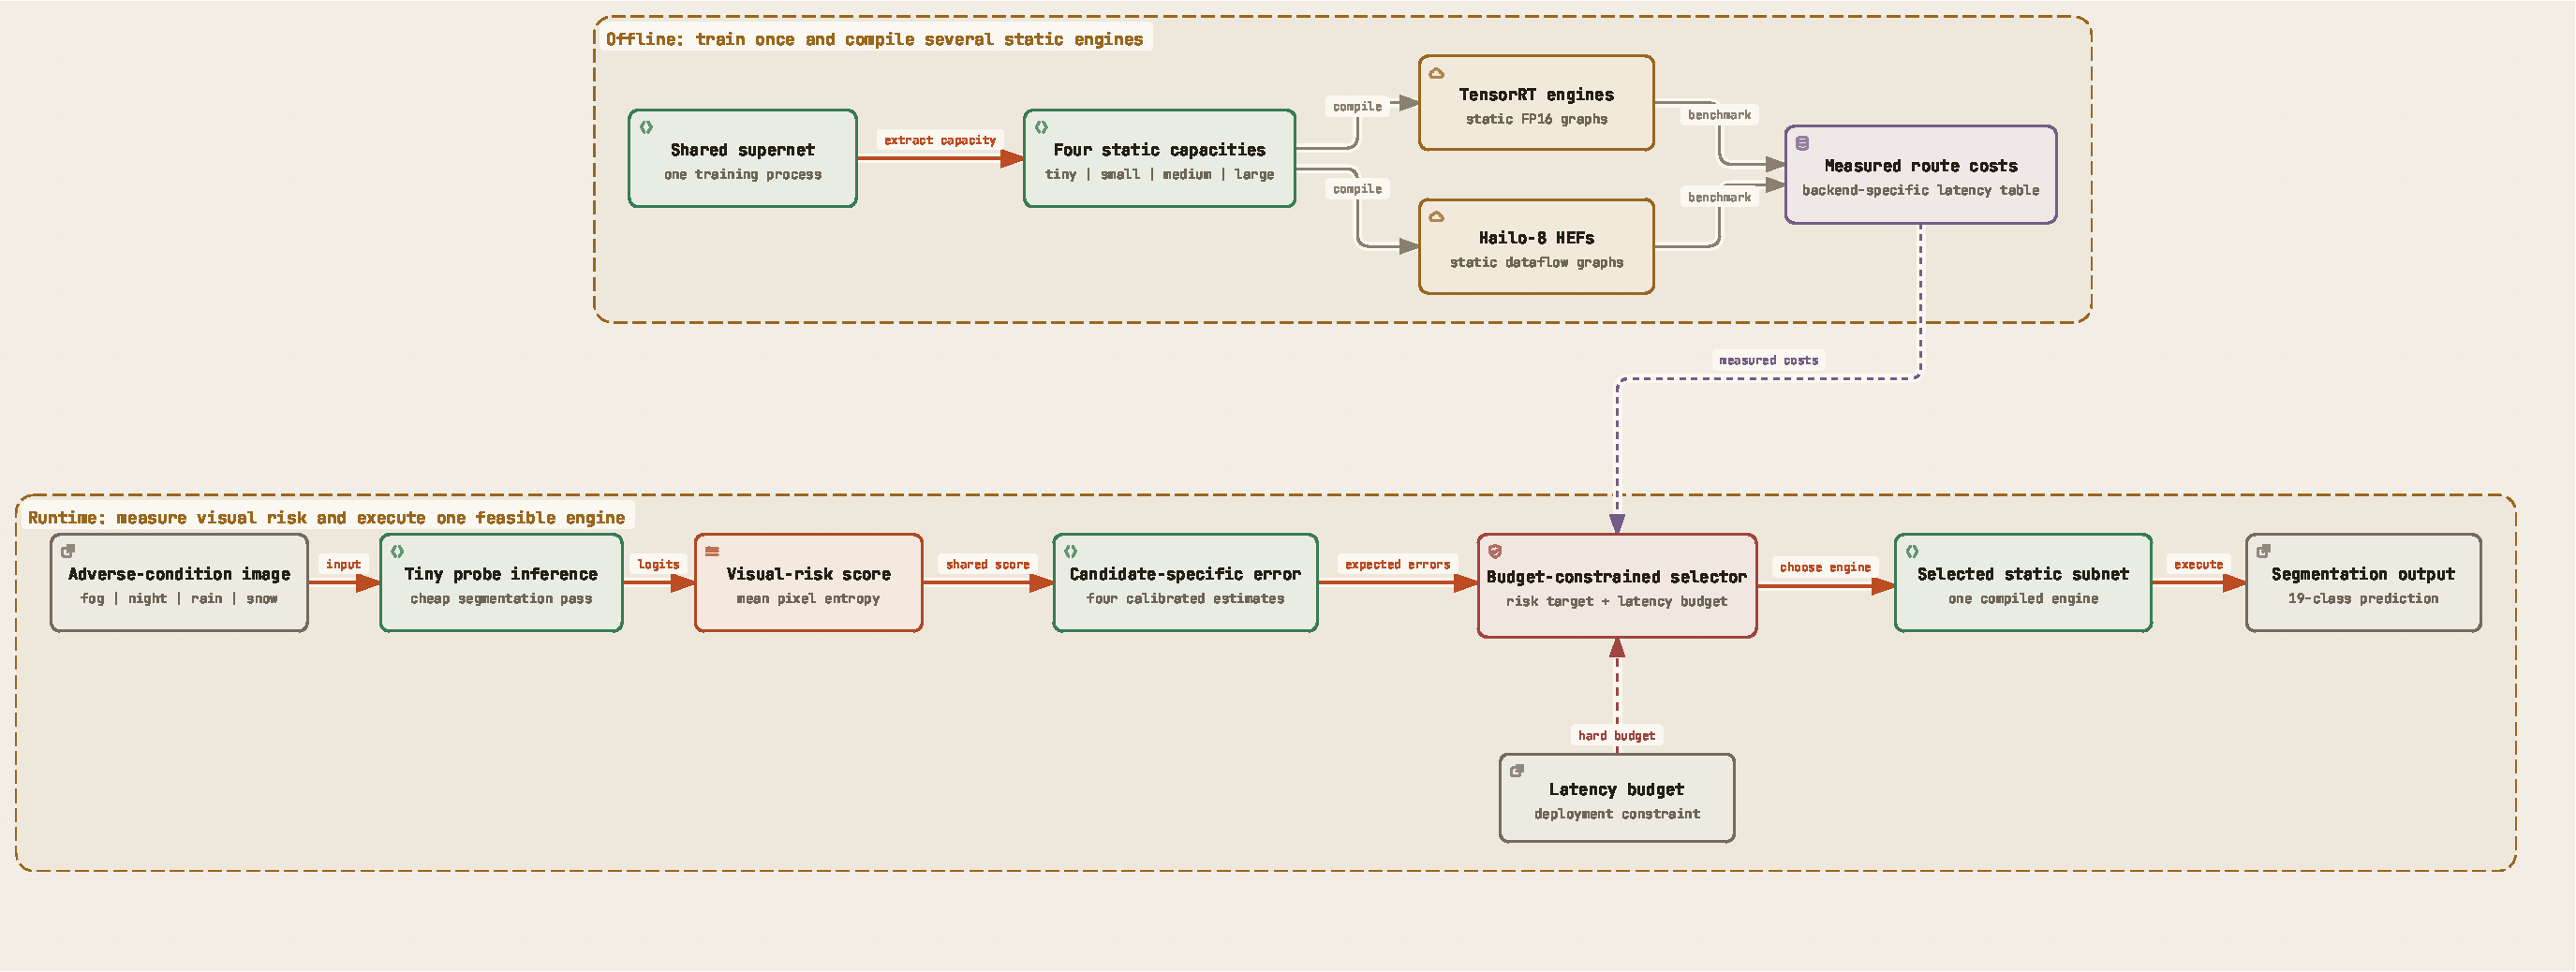
\includegraphics[width=\textwidth]{figures/fig1_pace_seg_system.pdf}
\caption{PACE-Seg separates offline candidate construction from runtime selection. One shared supernet yields four static capacities that are compiled and benchmarked for each backend. At runtime, the tiny candidate supplies a segmentation probe; one shared entropy score is mapped to four candidate-specific expected errors, and measured route costs plus a latency budget determine which static engine executes. The figure distinguishes training once, compiling several fixed graphs, and selecting one graph per image.}
\label{fig:overview}
\end{figure*}

\subsection{Compiler-safe elastic candidate family}
\label{sec:elastic}

\method{} contains four discrete levels: tiny, small, medium, and large. Their width multipliers are 0.25, 0.50, 0.75, and 1.00; their repeated block counts are 2, 3, 4, and 6; and their input resolutions are $384\times192$, $512\times256$, $768\times384$, and $1024\times512$ pixels. The levels share convolutional weights through active-channel slicing and use level-specific batch-normalization state. The operator set is restricted to convolutions, normalization, standard activations, pooling, elementwise operations, concatenation, and static-factor bilinear resizing that passed compiler smoke tests in the evaluated toolchains. Because no unconstrained-operator control was trained, compiler compatibility is deployment evidence rather than a measured accuracy contribution.

The four levels are exported as separate static graphs. Runtime routing therefore selects an engine before the selected candidate is executed; no compiled graph contains data-dependent control flow.

\begin{figure*}[t]
\centering
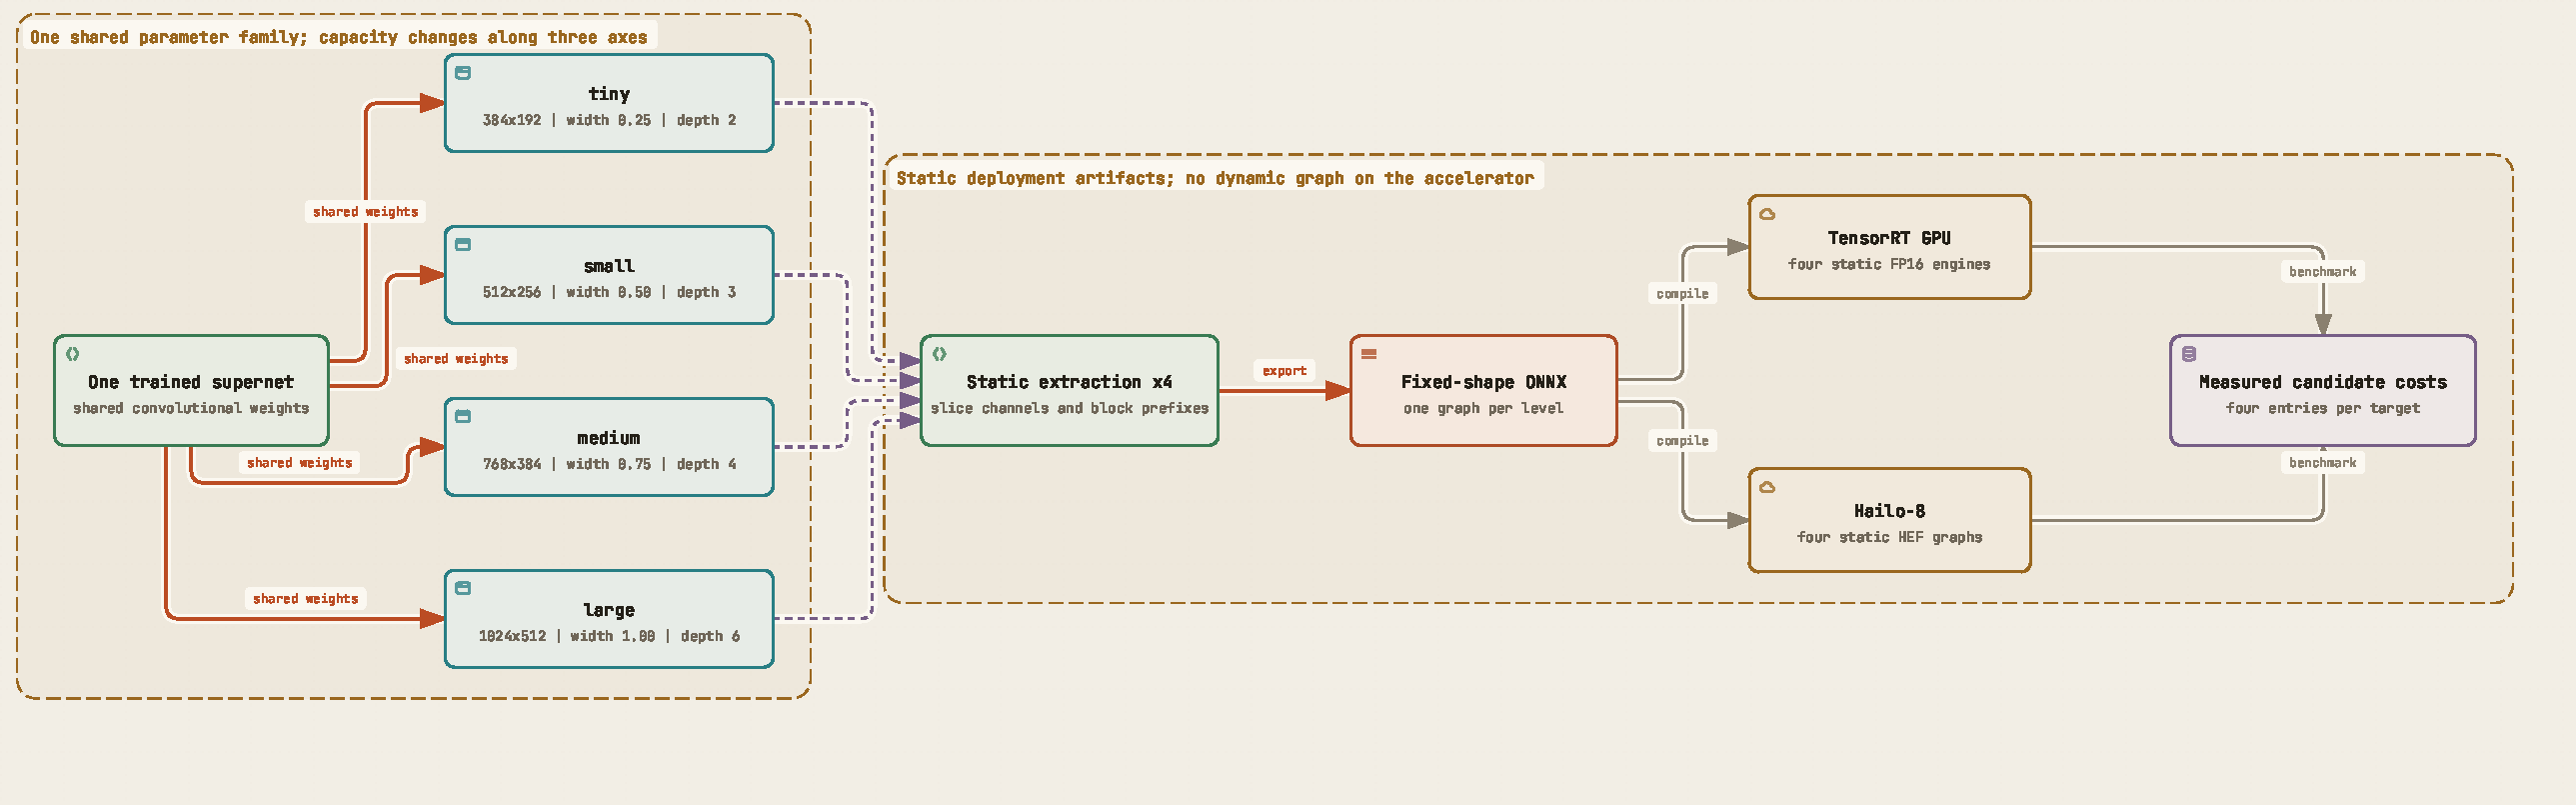
\includegraphics[width=\textwidth]{figures/fig2_elastic_deployment.pdf}
\caption{Elasticity and deployment portability. Tiny, small, medium, and large share one parameter family but differ jointly in input resolution, active width, and active depth. Static extraction slices channels and block prefixes before fixed-shape ONNX export, after which TensorRT and Hailo compile four independent accelerator graphs. Runtime hardware cost is consequently measured for each compiled candidate rather than inferred from the shared training graph.}
\label{fig:elastic-deployment}
\end{figure*}

\subsection{Measured-cost candidate set}
\label{sec:measured-cost}

For target hardware $h$, each candidate $l$ has a measured route cost $t_{h,l}$. Candidate-only measurements characterize the hardware ordering and Pareto set. Runtime measurements include the complete decision path: tiny probe inference, entropy computation, policy evaluation, engine activation or dispatch, and any additional candidate inference. The tiny prediction is reused when the policy selects tiny.

Measured cost enters the policy after training. It does not alter supernet optimization and therefore should not be interpreted as hardware-aware training or continuous architecture search. A new target requires a four-entry measured cost table, not retraining the segmentation model.

\subsection{Candidate-specific visual-risk calibration}
\label{sec:calibration}

Let the tiny candidate produce logits $z(x)$. The raw probe score is mean pixel entropy,
\begin{equation}
s(x)=\frac{1}{|\Omega|}\sum_{u\in\Omega}-\sum_{c=1}^{C}p_{u,c}\log\max(p_{u,c},10^{-12}),
\label{eq:entropy}
\end{equation}
where $p$ is the softmax of $z$ and $C=19$. The score is image-level and requires no separate probe network.

For each candidate $l$, we fit a monotonic calibrator $g_l$ that maps the same $s(x)$ to the candidate's observed per-image pixel error. The entropy feature is computed over all output pixels during fitting and deployment. Ground truth is used only to compute the fit-half error target over non-ignore labels. Fit-half samples are divided into ten equal-count bins by probe score. The target in each bin is the mean observed error of candidate $l$, and a cumulative-maximum pass enforces non-decreasing expected error. Thus
\begin{equation}
\widehat{r}_l(x)=g_l(s(x))
\label{eq:risk}
\end{equation}
is candidate-specific calibration from shared sensing, not candidate-specific probing. The primary analysis fits a separate calibrator set for Cityscapes and each ACDC condition and therefore assumes that the condition is configured. A second variant pools every split's fit half into one calibrator set and requires no condition choice at inference. Both use the same all-pixel entropy feature and the same held-out protocol.

\subsection{Hardware-cost-conditioned policy}
\label{sec:policy}

For a target device, candidate $l$ has measured route cost $t_l$, risk target $\tau$, and budget $B$. The proposed policy D forms the feasible set
\begin{equation}
\mathcal{S}_B=\{l:t_l\leq B\}.
\label{eq:feasible}
\end{equation}
If at least one feasible candidate satisfies $\widehat{r}_l(x)\leq\tau$, D selects the cheapest such candidate. Otherwise it selects the feasible candidate with minimum predicted error, breaking ties by lower cost. If no candidate is within budget, it selects the globally cheapest candidate. This fallback can still exceed a budget smaller than the cheapest available route; the evaluated budget grid uses the four measured route costs, so this case does not occur in the reported cells.

We compare D with three progressive ablations. A uses one calibrator for the probe candidate and escalates by latency rank according to integer multiples of $\tau$. B retains the single risk value but targets a latency magnitude before choosing the closest candidate. C uses candidate-specific risks but has no explicit budget. The progression is not a factorial $2\times2$ because D adds a hard-budget axis absent from A--C. We additionally run D with calibrators pooled across conditions. Static candidates, uncalibrated entropy routing, and a ground-truth oracle are references. The oracle is used only as an upper bound and never supplies information to a deployable policy.

\subsection{Implementation details and secondary QAT study}
\label{sec:qatmethod}

Elastic training uses the sandwich rule: each step evaluates the smallest and largest levels and one randomly selected intermediate level. The largest level receives supervised segmentation loss; smaller levels receive supervised and in-place distillation terms; and a boundary auxiliary term emphasizes semantic transitions. Training uses 100,000 optimization steps, batch size 8, AdamW with weight decay $10^{-4}$, initial learning rate $3\times10^{-4}$, cosine decay, 500 warm-up steps, and gradient clipping at 5.0. The data stream combines Cityscapes and ACDC with random scale/crop/pad, horizontal flip, and color jitter.

QAT replaces each convolution with per-tensor symmetric 8-bit fake quantization of its input activation and active weight tensor, using PyTorch's straight-through estimator. Dynamic mode derives the activation scale from every call. Calibrated mode freezes one activation range per layer after a 200-image calibration pass spanning clean and adverse conditions. The maximum observer retains the largest activation observed over all calls. The EMA-percentile observer computes the 99.9th percentile of absolute activation in each call and combines successive values with momentum 0.9.

For a slimmable convolution, one calibration buffer belongs to the shared layer and aggregates calls from all elasticity levels; the implementation does not maintain a separate frozen activation scale for each level. Each QAT run fine-tunes 10,000 steps from an FP32 checkpoint at learning rate $3\times10^{-5}$. These are simulated fake-quant results. They neither execute integer kernels nor establish compiled TensorRT or Hailo INT8 accuracy.

\section{Experimental protocol}
\label{sec:protocol}

\subsection{Datasets and splits}

Cityscapes supplies 2,975 training and 500 validation images~\cite{cordts2016cityscapes}. ACDC supplies 1,600 training and 406 validation images distributed across fog, night, rain, and snow~\cite{sakaridis2021acdc}. Both use the 19 Cityscapes train classes. Each validation split is partitioned by alternating index: even-index images form the calibration and operating-point fit half, and odd-index images form the held-out evaluation half. The study does not use an external test server.

\subsection{Training runs and baselines}

The near-parity comparison uses three reported supernet runs and three augmented Fast-SCNN runs. The router analysis uses the three separately trained checkpoints summarized in Table~\ref{tab:provenance}. The deployment-matched artifacts record each checkpoint SHA-256 and its embedded configuration hash. Initialization-parent identifiers and immutable full training manifests remain unavailable, so we call them separate training runs rather than a controlled identical-configuration seed study.

\begin{table}[H]
\centering
\caption{Training-checkpoint provenance used by the router analysis. Hashes are abbreviated; full SHA-256 values and remaining provenance boundaries are retained in the evidence manifest.}
\label{tab:provenance}
\small
\begin{tabularx}{\textwidth}{@{}lXlll@{}}
\toprule
Run & Training record & Step & Checkpoint SHA & Config hash \\
\midrule
A & Augmentation-labelled & 100,000 & \texttt{a2444156} & \texttt{6d1274f40e43} \\
B & Earlier unlabelled & 100,000 & \texttt{00da283c} & \texttt{837cf981427a} \\
C & Augmentation-labelled & 100,000 & \texttt{275dfcbf} & \texttt{ac52eabac3de} \\
\bottomrule
\end{tabularx}
\end{table}

Fixed-architecture comparisons cover Fast-SCNN, BiSeNetV2, SegFormer-B0, DDRNet-23-slim, and MobileNetV3/DeepLabV3. Fast-SCNN is the parameter-matched RQ2 comparator for the large elastic level. Routing references comprise static candidates, raw entropy, rank-based policy A, latency-spacing policy B, candidate-specific policy C without a budget, condition-specific and pooled variants of constrained policy D, and an oracle.

\subsection{Hardware and compiler versions}

Table~\ref{tab:hardware} identifies the four latency targets and their compiler stacks. TensorRT measurements use GPU FP16. Hailo candidates are compiled from ONNX through Hailo's Dataflow Compiler to HEF. Compiler smoke tests establish that all four static candidates execute on the primary TensorRT GPU and Hailo paths; DLA is excluded from headline analysis because decoder execution falls back to the GPU.

\begin{table}[H]
\centering
\caption{Hardware and compiler stacks used for candidate-latency measurement. Versions are reported because engine behavior is toolchain-specific.}
\label{tab:hardware}
\small
\begin{tabularx}{\textwidth}{@{}llX@{}}
\toprule
ID & Hardware & Runtime and system versions \\
\midrule
E1 & Raspberry Pi 5 + Hailo-8 M.2 & HailoRT 4.23.0; HEFs produced with Dataflow Compiler 3.34.0 and Model Zoo 2.19.0 \\
E2 & Jetson Xavier NX & L4T R35.4.1; CUDA 11.4.19; cuDNN 8.6.0.166; TensorRT 8.5.2.2 \\
E3 & Jetson AGX Xavier & L4T R35.6.4; CUDA 11.4.19; TensorRT 8.5.2.2 \\
E5 & Jetson Orin Nano Super & L4T R36.5.0; CUDA 12.6.68; cuDNN 9.3.0; TensorRT 10.3.0.30 \\
\bottomrule
\end{tabularx}
\end{table}

\subsection{Latency protocol}

Candidate-only latency is measured on four devices: E1, a Raspberry Pi 5 host with a Hailo-8 M.2 accelerator; E2, a Jetson Xavier NX; E3, a Jetson AGX Xavier; and E5, a Jetson Orin Nano. NVIDIA devices use TensorRT FP16. Measurements use batch size one, warm-up, three independent benchmark runs for the candidate lookup table, and bootstrap intervals. Energy is excluded because no external calibrated power meter was available.

Complete warm route costs are measured on E1 and E3. On E3, all four TensorRT contexts are resident; route timing includes tiny inference, device-resident entropy, policy evaluation, dispatch, and additional candidate inference. On E1, route timing includes mandatory network-group activation and deactivation, tiny inference, host entropy, policy evaluation, and additional candidate inference. Each route class uses 50 warm-up iterations and at least 500 timed iterations. Tiny output is reused when tiny is selected. Backend-specific cold-start measurements are excluded because the two runtimes impose different reload semantics.

The route harnesses use compiled graphs with the correct post-rescale architecture but do not execute trained checkpoint weights for the accuracy evaluation. The analysis combines measured route latency with cached trained-model predictions in an offline, per-image policy replay. It is not an integrated on-device accuracy run.

\subsection{Metrics, seed policy, and unit of analysis}

Segmentation quality is dataset-level \miou{}. Router calibration targets per-image pixel error, while routed quality is recomputed by accumulating confusion matrices from the selected candidates and calculating \miou{} once over the routed held-out set. Headline accuracy comparisons require three training runs. The router evidence uses Runs A--C, but incomplete configuration provenance prevents treating them as a perfectly controlled identical-configuration seed study.

The router reporting unit is an operating cell defined by checkpoint, backend cost table, dataset split, and budget. Cells reuse images, predictions, thresholds, and candidate sets. They are correlated analysis points, not independent statistical samples. We therefore report descriptive counts and macro averages without cell-level $p$-values or confidence intervals.

A fair A-versus-D cell is one in which A has zero held-out per-image budget violations at its fit-selected operating point. An operating cell is violating when at least one held-out image exceeds its budget. Fair-cell quality counts are always paired with violation counts over the full grid. D's zero violating-cell count is partly structural because D removes candidates above budget.

\subsection{Fit/held-out separation and leakage safeguards}
\label{sec:split}

Every candidate is evaluated once per image and its prediction is cached. The probe feature is mean softmax entropy over all output pixels in both fitting and deployment. Within each dataset split, condition-specific calibrators use only fit-half probe scores and candidate errors; the pooled variant combines only those fit halves across the five splits. Five risk targets are the 10th, 25th, 50th, 75th, and 90th percentiles of fit-half observed error, macro-aggregated across the five splits. One grid is generated per checkpoint and reused across E1 and E3 cost tables.

For each budget and policy, the representative risk target is selected from fit-half statistics: among points whose fit-half mean cost satisfies the budget, the procedure chooses the highest fit-half \miou{} and breaks ties by lower cost. Held-out outcomes are read only after this choice. The oracle uses held-out ground truth only as a non-deployable upper bound.

Held-out labels do not fit calibrators, define thresholds, or select operating points. They are used only to reconstruct final routed \miou{} and to report per-image budget violations after selection. The all-pixel probe feature requires no ground-truth mask at deployment. The historical masked-fit artifacts are retained for audit but are not used for the RQ3 headline.

\section{Results}
\label{sec:results}

\subsection{RQ1: Why measured hardware cost is necessary}

The four levels require 0.2060, 1.1678, 6.1712, and 22.6992 GFLOPs. Their large-to-tiny ratio is 110.2, whereas measured mean end-to-end candidate latency grows by only $10.3$--$19.5\times$ across the four accelerators (Fig.~\ref{fig:flops-latency}). A 10~ms budget selects small on E1/E2, large on E3, and medium on E5. Measured cost is therefore necessary to recover hardware feasibility in this candidate set. The result concerns a proportional FLOPs proxy; it does not establish that learned latency predictors or FLOPs-aware search fail in general.

\begin{figure*}[t]
\centering
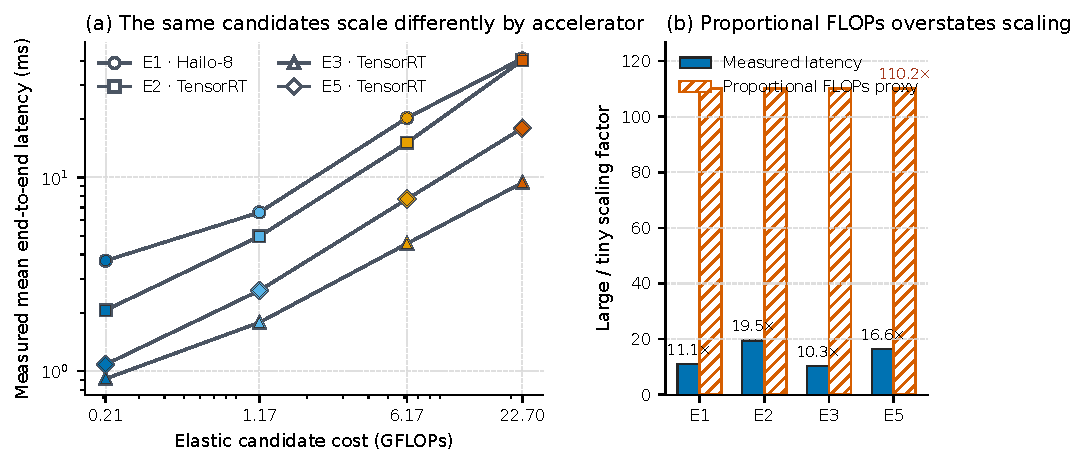
\includegraphics[width=\textwidth]{figures/fig3_flops_vs_latency.pdf}
\caption{Why FLOPs is insufficient as a deployment-cost proxy. (a) The four elastic levels are plotted at their actual GFLOPs and measured mean end-to-end latency on E1, E2, E3, and E5; marker shape identifies hardware and marker color identifies capacity. (b) Large increases compute by $110.2\times$ relative to tiny, but measured latency increases by only $10.3$--$19.5\times$, depending on the accelerator. FLOPs preserves the candidate order here but not the hardware-specific cost scale required by a latency budget.}
\label{fig:flops-latency}
\end{figure*}

The budget sweep confirms that the mismatch affects selection rather than only scale. Across 640 proxy evaluations, same-device proportional fits mis-select 37.5--65\% of budgets, and the worst cross-device transfers reach 85--95\% mis-selection or violation. Measured cost is therefore required for this candidate set. The sweep does not compare against learned latency predictors.

\subsection{RQ2: Whether shared elastic training preserves quality}

The elastic model preserves matched-capacity segmentation quality across clean and adverse conditions. Across the three reported runs per model, the large level differs from a similarly sized independently trained Fast-SCNN by +1.10, +0.21, $-0.65$, $-0.23$, and +0.07 \miou{} points on Cityscapes, fog, night, rain, and snow, respectively (Fig.~\ref{fig:rq2}). Every observed mean difference remains within the prespecified $\pm1.5$-point practical near-parity band, and the run envelopes cross zero on four of five splits. This supports practical near-parity rather than superiority. The comparison does not measure total training, packaging, or maintenance savings.

\begin{figure*}[t]
\centering
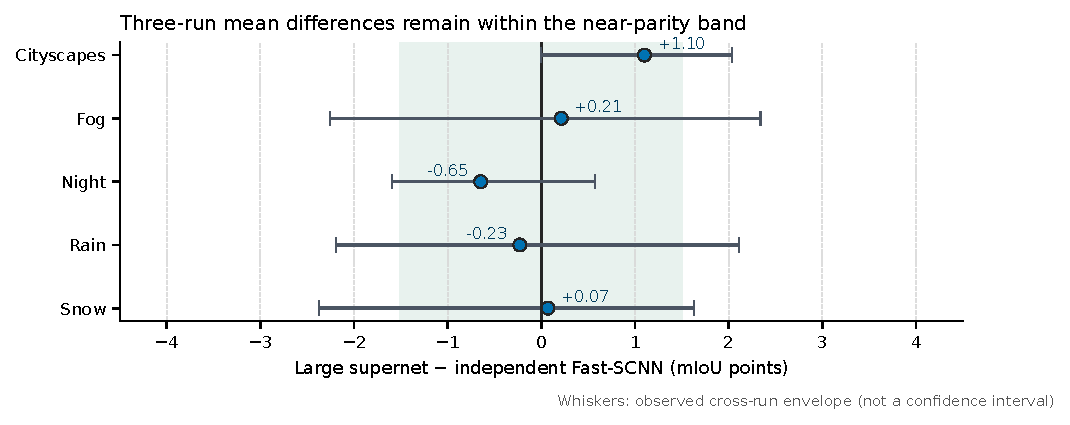
\includegraphics[width=\textwidth]{figures/fig4_rq2_near_parity.pdf}
\caption{Three-run matched-capacity comparison. Points are differences between the mean \miou{} of the large elastic candidate and independently trained Fast-SCNN; positive values favor the elastic candidate. Whiskers show the full observed cross-run envelope formed from the two three-run sets and are descriptive, not confidence intervals or paired-seed estimates. Every observed mean remains inside the prespecified $\pm1.5$-point practical near-parity band; this does not establish superiority or statistical equivalence.}
\label{fig:rq2}
\end{figure*}

\subsection{RQ3: Candidate-specific routing under measured budgets}

The routing study tests whether candidate-specific expected-error estimates improve budget-constrained selection over a single-score rank policy. An earlier candidate-only ablation supports the progression from A to D, but it omits complete route overhead and predates deployment-matched calibration. We therefore use it only as mechanism-level directional evidence and base the RQ3 conclusion on the corrected complete-route replay below.

\subsubsection{Measured route costs}

Complete route costs materially exceed candidate-only inference costs, and the dominant source depends on the accelerator. Table~\ref{tab:routes} reports the warm-route medians used in the overhead-aware replay; every value includes the tiny probe, risk evaluation, policy decision, switching or activation, and any additional candidate inference.

\begin{table}[H]
\centering
\caption{Median warm end-to-end route cost used in the overhead-aware replay.}
\label{tab:routes}
\begin{tabular}{@{}lrr@{}}
\toprule
Route & E3 TensorRT/CUDA & E1 Hailo-8 \\
\midrule
tiny $\rightarrow$ tiny & 2.07 ms & 34.95 ms \\
tiny $\rightarrow$ small & 5.23 ms & 46.13 ms \\
tiny $\rightarrow$ medium & 11.97 ms & 63.36 ms \\
tiny $\rightarrow$ large & 26.70 ms & 92.68 ms \\
\bottomrule
\end{tabular}
\end{table}

On E3, complete routes range from 2.07 to 26.70~ms; on E1 they range from 34.95 to 92.68~ms. Host-side uncertainty evaluation is the main avoidable cost on E3, whereas network-group activation dominates E1. A production-path audit on 40 TensorRT outputs measures a maximum risk-score deviation of $7.15\times10^{-7}$ nats from the PyTorch reference, below the prespecified $10^{-4}$ tolerance. The measurements show that candidate-only lookup tables omit substantial, backend-specific costs. They cover two warm execution paths and do not establish equivalent cold-start semantics across the backends.

\subsubsection{Deployment-matched routing result}

The overhead-aware replay recomputes A and D decisions with measured warm route costs, constructs each backend's budget grid from its four route costs, and selects risk targets using fit-half data. One canonical risk grid per training run is shared across E1 and E3. The probe feature is identical at fitting and deployment. We report both configured condition-specific D and pooled D, which fits one candidate-calibrator set from all five fit halves.

\begin{table}[H]
\centering
\caption{Deployment-matched A-versus-D comparison with measured complete route costs. W/T/L uses fair cells; violations use the full grid. Pooled D uses one calibrator set across conditions.}
\label{tab:routerfinal}
\footnotesize
\setlength{\tabcolsep}{3.5pt}
\begin{tabular}{@{}llrrrrrr@{}}
\toprule
Policy & Backend & Fair & W/T/L & Win/tie & Mean $\Delta$ & Policy viol. & A viol. \\
\midrule
Configured D & E3 & 38/60 & 29/7/2 & 94.7\% & +0.0287 & 0/60 & 22/60 \\
Configured D & E1 & 36/60 & 27/7/2 & 94.4\% & +0.0279 & 0/60 & 24/60 \\
Configured D & Overall & 74/120 & 56/14/4 & 94.6\% & +0.0284 & 0/120 & 46/120 \\
Pooled D & Overall & 74/120 & 58/14/2 & 97.3\% & +0.0296 & 0/120 & 46/120 \\
\bottomrule
\end{tabular}
\end{table}

\begin{figure*}[t]
\centering
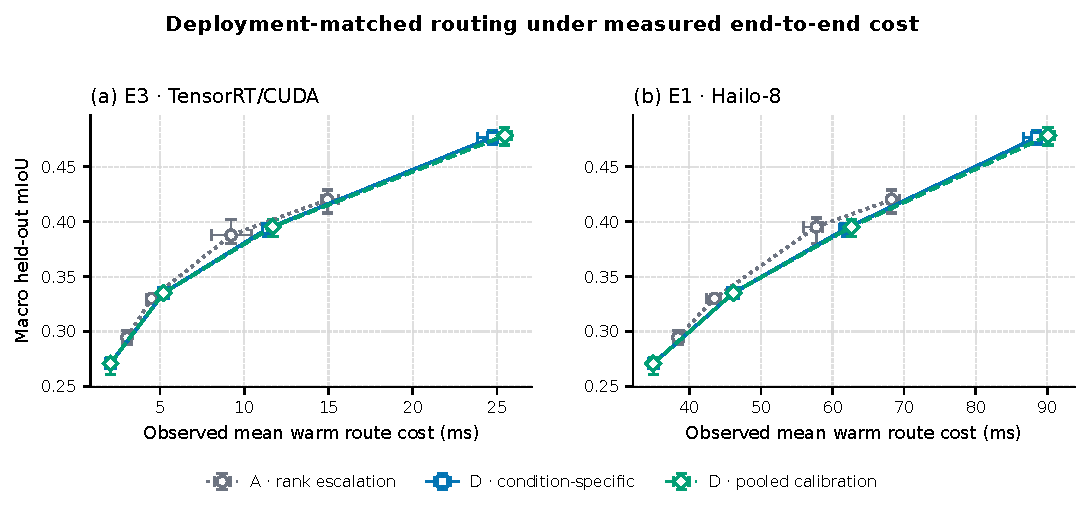
\includegraphics[width=\textwidth]{figures/fig5_router_deployment_matched.pdf}
\caption{Quality versus measured complete warm-route cost after deployment-matched calibration. Each point first macro-averages the five held-out splits within one training run and then averages Runs A--C; horizontal and vertical whiskers show the full run-level range, not confidence intervals. Points are placed at observed mean route cost rather than nominal budget. Both candidate-specific hard-budget variants extend to higher-quality operating points than rank policy A; pooled calibration closely tracks configured condition-specific calibration on E3 and E1.}
\label{fig:router-frontier}
\end{figure*}

Under this protocol, configured D outperforms or matches A in 70 of 74 fair cells (56 wins, 14 ties, and 4 losses), with a macro D-minus-A gap of +0.0284 \miou{}. Across the full 120-cell grid, D has no budget-violating operating point and A has 46. Pooled D records 58 wins, 14 ties, and 2 losses on the same fair subset, with a +0.0296 gap. The similar curves in Fig.~\ref{fig:router-frontier} show that candidate-specific hard-budget selection, rather than per-condition calibrator choice, drives the observed gain.

The 74 fair cells are the subset in which A satisfies its own budget; they are correlated operating points rather than independent trials. D's zero-violation count follows partly from enforcing feasibility by construction, and E1 and E3 share segmentation predictions. The cross-backend comparison therefore tests the effect of different measured cost tables, not independent accuracy replication. Absolute hardware costs determine feasibility and latency, but identical candidate ordering can still produce identical decisions.

\subsection{Adverse-condition behavior}

Adverse conditions affect both segmentation quality and the informativeness of the shared probe. Across Runs A--C, the large elastic level averages 0.5311 \miou{} on the held-out Cityscapes half but 0.3559 on ACDC/night. Probe-signal AURC averages 0.1411 across the fifteen run--split evaluations and is worst at night, where the three-run mean is 0.2416. Night imagery therefore weakens both prediction quality and uncertainty ranking. These are descriptive values on the evaluated validation halves.

Configured D's four fair-cell losses arise from two Run C operating points---fog and rain at the medium budget---replayed on both backends. Pooled D's two small losses are the same Run B snow operating point replayed on E1 and E3. The duplication follows shared predictions and should not be interpreted as independent failures or a failure probability.

\subsection{Secondary deployment and fake-quant evidence}
\label{sec:qatresults}

All four static candidate graphs compile and execute through TensorRT and Hailo-8 deployment paths. This establishes compiler compatibility for the constrained operator set, but the study has no trained unconstrained control and therefore does not attribute an accuracy benefit to compiler safety.

Observer choice controls the worst adverse-condition degradation in the fake-quant study. Dynamic fake quantization of the shared large level loses 1.66, 2.54, and 1.39 \miou{} points in the worst condition of the three runs, whereas EMA-percentile calibration produces the bounds in Table~\ref{tab:qat}. A Run A $2\times2$ comparison indicates a larger change from the observer than from subnet export. Because the identity of the worst condition can differ between cells and mean effects are not uniformly positive, the comparison does not establish additive causal effects.

\begin{table}[H]
\centering
\caption{Absolute worst-condition \miou{} degradation under shared-supernet EMA-percentile fake-quant QAT.}
\label{tab:qat}
\begin{tabular}{@{}lrrrr@{}}
\toprule
Training run & tiny & small & medium & large \\
\midrule
Run A & 0.32 & 0.97 & 0.51 & 0.97 \\
Run B & 0.69 & 0.33 & 0.49 & 1.38 \\
Run C & 0.36 & 0.33 & 0.56 & 0.86 \\
\bottomrule
\end{tabular}
\end{table}

Every evaluated run and level remains within 1.5 points, and the worst large-level run improves from 2.54 to 1.38 points. EMA-percentile calibration therefore stabilizes worst-condition fake-quant degradation in this setting. Mean quality is not consistently improved, activation outlier suppression remains an untested explanation, and no compiled INT8 accuracy claim follows.

\section{Discussion}
\label{sec:discussion}

The experiments separate candidate construction, hardware feasibility, and image-dependent selection. Shared elastic training supplies four static candidates without a large quality penalty at matched capacity. Direct measurement then defines which candidates fit a deployment budget. Candidate-specific calibration finally estimates whether additional capacity is warranted for an image. Treating these as distinct decisions makes clear which evidence supports each part of the system.

FLOPs fails here primarily as a cost scale rather than an ordering statistic. The 110.2-fold compute range contracts to a 10.3--19.5-fold latency range because operators, memory behavior, compiler mappings, and accelerator execution differ. A ranking may therefore transfer when candidate order is preserved, while budget feasibility still changes with absolute measured cost. This explains why some routing decisions coincide across devices without making the cost table dispensable.

Candidate-specific calibration addresses a limitation of a single probe score: equal probe entropy need not imply equal error for every candidate. The deployment-matched results are consistent with this premise, but calibration cannot recover visual information absent from the probe. ACDC/night has the weakest uncertainty ordering even though the residual paired losses occur in other conditions. Pooled calibration matches or slightly exceeds configured condition-specific calibration, so condition-specific fitting is not necessary for the reported result; generalization to conditions absent from the calibration pool remains untested.

Complete route measurement changes the deployment conclusion. Candidate-only inference time omits uncertainty computation and accelerator-specific switching or activation. These omissions are large on both evaluated backends even though their causes differ. Hardware-aware runtime selection should therefore account for the complete route path, not only isolated candidate latency.

The quantization study reinforces the need to separate measurement from mechanism. Percentile/EMA calibration reduces worst-condition fake-quant degradation across the tested runs and levels, but the data do not directly measure activation outliers or compiled integer behavior. QAT consequently remains secondary deployment evidence rather than a primary contribution.

\section{Limitations and threats to validity}
\label{sec:limitations}

First, calibration is evaluated only on Cityscapes and the four ACDC conditions. The configured variant assumes that the condition is known, while the pooled variant removes that runtime choice but still uses fit-half samples from every evaluated condition. Neither result establishes calibration on a previously unseen adverse condition.

Second, the evaluation uses alternating halves of validation splits rather than an external test set. Multiple budgets and thresholds reuse the same images and predictions. Operating cells are correlated, and the 120-cell denominator is not a statistical sample size. Runs A--C form the training-replication axis. Checkpoint and embedded configuration hashes are recorded, but initialization-parent provenance is incomplete.

Third, fair-cell conditioning is descriptive. It excludes A's budget-violating comparisons so that quality is compared only when A honors its contract, but the denominator depends on baseline behavior. Full-grid violation counts must accompany the fair-cell result. D's zero violations are partly guaranteed by construction and are not empirical reliability.

Fourth, E1 and E3 share segmentation predictions. Separately measured route-cost tables are combined with the same per-image prediction caches. The compiled timing engines have the correct architecture but are not the trained engines that produced accuracy. The study validates cost accounting and overhead-aware replay, not bit-exact compiled-model accuracy or a continuously running application.

Fifth, breakpoint budgets can reduce hardware conditioning to latency rank. Absolute costs change feasibility and mean-latency operating-point selection, but identical orderings can produce identical route choices. Hardware-cost-conditioned describes the policy input; it does not imply device-specific decisions in every case.

Sixth, QAT uses fake quantization in PyTorch. No compiled INT8 accuracy, integer-kernel speedup, or backend-specific quantization behavior is established. The observed EMA-percentile result is consistent with reduced outlier sensitivity but does not measure that mechanism directly.

Finally, the study uses four candidates, two complete route-cost backends, and no external power meter. It makes no energy claim. Temporal routing, unknown-condition calibration, cold-frontier behavior, uncertainty-aware segmentation metrics, and qualitative error analysis remain outside scope. The compiler-safe operator set was validated without a trained unconstrained control, so portability is an engineering property rather than an independently isolated accuracy contribution.

\section{Conclusion}
\label{sec:conclusion}

\method{} studies elastic semantic segmentation when both visual difficulty and accelerator cost vary. Measured latency is necessary to define feasible candidates, and shared elastic training preserves matched-capacity quality across the evaluated clean and adverse conditions. With deployment-matched calibration and complete warm-route costs, candidate-specific hard-budget routing improves the descriptive quality--cost trade-off over rank escalation on two structurally different accelerators. Pooled calibration retains the result without condition selection, while correlated cells, shared predictions, offline replay, and the absence of an external test set bound the claim.

\section*{Data and code availability}

The repository records the implementation, experiment reports, and canonical result artifacts. The accompanying evidence manifest maps Runs A--C to checkpoint and configuration hashes and traces each figure and numerical claim to its source artifact. The deployment-matched replay directory is the canonical RQ3 evidence; historical masked-fit replays remain available only for audit. Dataset access remains subject to the Cityscapes and ACDC licenses.

\begin{thebibliography}{99}

\bibitem{yu2018bisenet}
C. Yu, J. Wang, C. Peng, C. Gao, G. Yu, N. Sang,
BiSeNet: Bilateral segmentation network for real-time semantic segmentation,
in: European Conference on Computer Vision, 2018, pp. 325--341.
\url{https://openaccess.thecvf.com/content_ECCV_2018/html/Changqian_Yu_BiSeNet_Bilateral_Segmentation_ECCV_2018_paper.html}.

\bibitem{fan2021stdc}
M. Fan, S. Lai, J. Huang, X. Wei, Z. Chai, J. Luo, X. Wei,
Rethinking BiSeNet for real-time semantic segmentation,
in: IEEE/CVF Conference on Computer Vision and Pattern Recognition, 2021, pp. 9716--9725.
\url{https://openaccess.thecvf.com/content/CVPR2021/html/Fan_Rethinking_BiSeNet_for_Real-Time_Semantic_Segmentation_CVPR_2021_paper.html}.

\bibitem{xu2023pidnet}
J. Xu, Z. Xiong, S.P. Bhattacharyya,
PIDNet: A real-time semantic segmentation network inspired by PID controllers,
in: IEEE/CVF Conference on Computer Vision and Pattern Recognition, 2023, pp. 19529--19539.
\url{https://openaccess.thecvf.com/content/CVPR2023/html/Xu_PIDNet_A_Real-Time_Semantic_Segmentation_Network_Inspired_by_PID_Controllers_CVPR_2023_paper.html}.

\bibitem{xie2021segformer}
E. Xie, W. Wang, Z. Yu, A. Anandkumar, J.M. Alvarez, P. Luo,
SegFormer: Simple and efficient design for semantic segmentation with transformers,
Advances in Neural Information Processing Systems 34 (2021) 12077--12090.

\bibitem{zhang2025offseg}
S.-C. Zhang, Y. Li, Y.-H. Wu, Q. Hou, M.-M. Cheng,
Revisiting efficient semantic segmentation: Learning offsets for better spatial and class feature alignment,
in: IEEE/CVF International Conference on Computer Vision, 2025, pp. 22361--22371.
\url{https://openaccess.thecvf.com/content/ICCV2025/html/Zhang_Revisiting_Efficient_Semantic_Segmentation_Learning_Offsets_for_Better_Spatial_and_ICCV_2025_paper.html}.

\bibitem{yu2019slimmable}
J. Yu, L. Yang, N. Xu, J. Yang, T. Huang,
Slimmable neural networks,
in: ICLR Workshop, 2019.
\url{https://arxiv.org/abs/1812.08928}.

\bibitem{yu2019usnet}
J. Yu, T. Huang,
Universally slimmable networks and improved training techniques,
in: IEEE/CVF International Conference on Computer Vision, 2019, pp. 1803--1811.
\url{https://doi.org/10.1109/ICCV.2019.00189}.

\bibitem{cai2020ofa}
H. Cai, C. Gan, T. Wang, Z. Zhang, S. Han,
Once-for-All: Train one network and specialize it for efficient deployment,
in: International Conference on Learning Representations, 2020.
\url{https://openreview.net/forum?id=HylxE1HKwS}.

\bibitem{xue2022slimseg}
D. Xue, F. Yang, P. Wang, L. Herranz, J. Sun, Y. Zhu, Y. Zhang,
SlimSeg: Slimmable semantic segmentation with boundary supervision,
in: Proceedings of the 30th ACM International Conference on Multimedia, 2022, pp. 6539--6548.
\url{https://doi.org/10.1145/3503161.3548191}.

\bibitem{kouris2022mess}
A. Kouris, S.I. Venieris, S. Laskaridis, N.D. Lane,
Multi-exit semantic segmentation networks,
in: European Conference on Computer Vision, 2022, pp. 330--349.

\bibitem{li2020dynamic}
Y. Li, L. Song, Y. Chen, Z. Li, X. Zhang, X. Wang, J. Sun,
Learning dynamic routing for semantic segmentation,
in: IEEE/CVF Conference on Computer Vision and Pattern Recognition, 2020, pp. 8553--8562.

\bibitem{liu2022anytime}
Z. Liu, Z. Xu, H.-J. Wang, T. Darrell, E. Shelhamer,
Anytime dense prediction with confidence adaptivity,
in: International Conference on Learning Representations, 2022.
\url{https://openreview.net/forum?id=kNKFOXleuC}.

\bibitem{tan2019mnasnet}
M. Tan, B. Chen, R. Pang, V. Vasudevan, M. Sandler, A. Howard, Q.V. Le,
MnasNet: Platform-aware neural architecture search for mobile,
in: IEEE/CVF Conference on Computer Vision and Pattern Recognition, 2019, pp. 2820--2828.

\bibitem{chen2020fasterseg}
W. Chen, X. Gong, X. Liu, Q. Zhang, Y. Li, Z. Wang,
FasterSeg: Searching for faster real-time semantic segmentation,
in: International Conference on Learning Representations, 2020.
\url{https://openreview.net/forum?id=BJgqQ6NYvB}.

\bibitem{dou2023autosegedge}
Z. Dou, D.-Y. Ye, B. Wang, X. Wang, S. Sun,
AutoSegEdge: Searching for the edge device real-time semantic segmentation based on multi-task learning,
Image and Vision Computing 136 (2023) 104719.
\url{https://doi.org/10.1016/j.imavis.2023.104719}.

\bibitem{dou2024multiobjective}
Z. Dou, D.-Y. Ye, B. Wang, X. Wang, S. Sun,
Multi-objective neural architecture search for efficient and fast semantic segmentation on edge,
IEEE Transactions on Intelligent Vehicles 9 (1) (2024) 1346--1357.
\url{https://doi.org/10.1109/TIV.2023.3332594}.

\bibitem{li2023realtimeseg}
Y. Li, C. Yang, P. Zhao, G. Yuan, W. Niu, J. Guan, H. Tang, M. Qin, Q. Jin, B. Ren, X. Lin, Y. Wang,
Towards real-time segmentation on the edge,
Proceedings of the AAAI Conference on Artificial Intelligence 37 (2) (2023) 1339--1347.
\url{https://doi.org/10.1609/aaai.v37i2.25232}.

\bibitem{kwon2024hard}
Y. Kwon, W. Kim, H. Kim,
HARD: Hardware-aware lightweight real-time semantic segmentation model deployable from edge to GPU,
in: Asian Conference on Computer Vision, 2024, pp. 3552--3569.
\url{https://openaccess.thecvf.com/content/ACCV2024/html/Kwon_HARD__Hardware-Aware_lightweight_Real-time_semantic_segmentation_model_Deployable_from_ACCV_2024_paper.html}.

\bibitem{wang2023calibrating}
D. Wang, B. Gong, L. Wang,
On calibrating semantic segmentation models: Analyses and an algorithm,
in: IEEE/CVF Conference on Computer Vision and Pattern Recognition, 2023, pp. 23652--23662.

\bibitem{dejorge2023reliability}
P. de Jorge, R. Volpi, P.H.S. Torr, G. Rogez,
Reliability in semantic segmentation: Are we on the right track?,
in: IEEE/CVF Conference on Computer Vision and Pattern Recognition, 2023, pp. 2456--2465.

\bibitem{sakaridis2021acdc}
C. Sakaridis, D. Dai, L. Van Gool,
ACDC: The adverse conditions dataset with correspondences for semantic driving scene understanding,
in: IEEE/CVF International Conference on Computer Vision, 2021, pp. 10765--10775.

\bibitem{cordts2016cityscapes}
M. Cordts, M. Omran, S. Ramos, T. Rehfeld, M. Enzweiler, R. Benenson, U. Franke, S. Roth, B. Schiele,
The Cityscapes dataset for semantic urban scene understanding,
in: IEEE Conference on Computer Vision and Pattern Recognition, 2016, pp. 3213--3223.

\bibitem{xu2023eqnet}
S. Xu, Y. Li, M. Lin, P. Gao, G. Guo, J. Lue, B. Zhang,
EQ-Net: Elastic quantization neural networks,
in: IEEE/CVF International Conference on Computer Vision, 2023, pp. 15072--15082.

\bibitem{jin2020adabits}
Q. Jin, L. Yang, Z. Liao,
AdaBits: Neural network quantization with adaptive bit-widths,
in: IEEE/CVF Conference on Computer Vision and Pattern Recognition, 2020, pp. 2146--2156.

\end{thebibliography}

\end{document}
